\documentclass[../all.tex]{subfiles}
\begin{document}
%%%%%%%%%%%%%%%%%%
    \section{Sports Fake Detector}
%%%%%%%%%%%%%%%%%%

\subsection{Tecnologías utilizadas}
    \subsubsection{MongoDB}
        MongoDB es un sistema de bases de datps NoSql de código abierto orientado a documentos. En lugar de almacenar la información en tablas como se haría en una base de datos relacional, MongoDB guarda la información en forma de documentos JSON, haciendo que la integración de este sistema de información sea mucho más simple y rápido que otros sistemas de bases de datos.\\
        MongoDB ha sido muy útil para almacenar de manera eficiente grandes conjuntos de tuits. Para trabajar con este sistema de bases de datos se ha empleado la líbreria PyMongo, que es la distribución para Python recomendada en la web oficial de MongoDB y que contiene todas las herramientas necesarias. Para el proyecto se ha empleado la versión 3.0.4 de MongoDB.\\
        MongoDB es un sistema fácil de utilizar y que funciona muy bien para guardar textos pero vamos a ver una tabla donde se puede comparar una base de datos como MongoDB con una SQL\footnote{Obtenida en \url{https://blog.pandorafms.org/es/bases-de-datos-nosql/}}.
        
    
        
        \begin{center}
            \begin{tabular}{ | m{3cm} | m{4cm}| m{4cm} | } 
                \hline
                \textbf{Feature} & \textbf{NoSQL Database} & \textbf{SQL Database} \\ 
                \hline
                Performance & High \checkmark & Low \\ 
                \hline
                Reliability & Poor & Good \checkmark \\ 
                \hline
                Availability & Good & Good \\ 
                \hline
                Consistency & Poor & Good \checkmark \\ 
                \hline
                Dara storage & Optimized for huge data \checkmark & Medium sized to large  \\ 
                \hline
                Scalability & High \checkmark & High but expensive  \\ 
                \hline
            \end{tabular}
        \end{center}
    \newpage
    \subsubsection{Pymongo 3.7.1}
        Pymongo es una librería de Python para poder conectarnos a una base de datos MongoDB.
        Para utilizar esta librería se utilizará una clase propia.
        \begin{figure}[H]
        	\centering
        	\includegraphics[height=13cm, width=15cm]{imgs/DB_class.png}
        	\caption{Clase DB utilizada para la comunicación entre el programa y la base de datos en MongoDB}
        \end{figure}
        
    \subsubsection{AVL Tree}
        
    	Todas las palabras están guardadas en una base de datos MongoDB pero con la finalidad de hacer la búsqueda más rápida una vez se consultan por primera vez se quedan guardadas en un árbol propio, concretamente en un AVL tree. \\
    	
    	Un árbol es un tipo abstracto de datos (TAD) muy utilizado que imita la estructura jerárquica de un árbol, con un valor en la raíz y subárboles con un nodo padre, representado como un conjunto de nodos enlazados.\\
   
    	La ventaja que tiene este tipo de árboles (AVL) es que están siempre equilibrados de tal modo que para todos los nodos, la altura de la rama izquierda no difiere en más de una unidad de la altura de la rama derecha o viceversa. Gracias a esta forma de equilibrio (o balanceo), la complejidad de una búsqueda en uno de estos árboles se mantiene siempre en orden de complejidad O(log n). El factor de equilibrio puede ser almacenado directamente en cada nodo o ser computado a partir de las alturas de los subárboles.\\
    	
    	\begin{figure}[H]
    		\centering
    		\includegraphics[height=10cm, width=13cm]{imgs/AVLtree_example.png}
    		\caption{Ejemplo AVL Tree}
    	\end{figure}
    	
    	Como se puede observar en la figura anterior, un árbol es unicamente una estructura de datos ordenada. En la figura es un orden numérico (de menos a más valor)  y el árbol utilizado en este trabajo está ordenado alfabéticamente. Con este árbol tendremos un coste inicial de creación pero luego el coste medio de la búsqueda de palabras será mucho menor.
    	\begin{figure}[H]
    		\centering
    		\includegraphics[height=13cm, width=11cm]{imgs/avl_class.png}
    		\caption{Diagrama de la clase propia AVL-TREE utilizada para la interacción con el árbol}
    	\end{figure}
    
\newpage
\subsection{Fase 0 - Extracción de la información y creación de los datasets}
    \subsubsection{Concepto}
        Esta primera fase o fase inicial se irá modificando al largo de la implementación según se necesite. Pretende englobar tanto la extracción de los tweets como la creación de los diccionarios.\\
        
        Se pretende así que cada deporte tenga tres diccionarios asociados (palabras excluyentes, palabras vinculantes principales y palabras vinculantes secundarias). También se tendrán diccionarios para el análisis de las frases; palabras vacías, que son aquellas palabras que no aportan nada a la hora de clasificar el texto como podrían ser artículos y preposiciones.Por último se tendrá un diccionario asociado a cada uno de los sentimientos a analizar; alegría, amor, enfado, miedo, sorpresa y tristeza.
   \newpage 
    \subsubsection{Software}
        El esquema de esta fase se puede ver en la siguiente imagen:\\
        \begin{figure}[H]
        \centering
            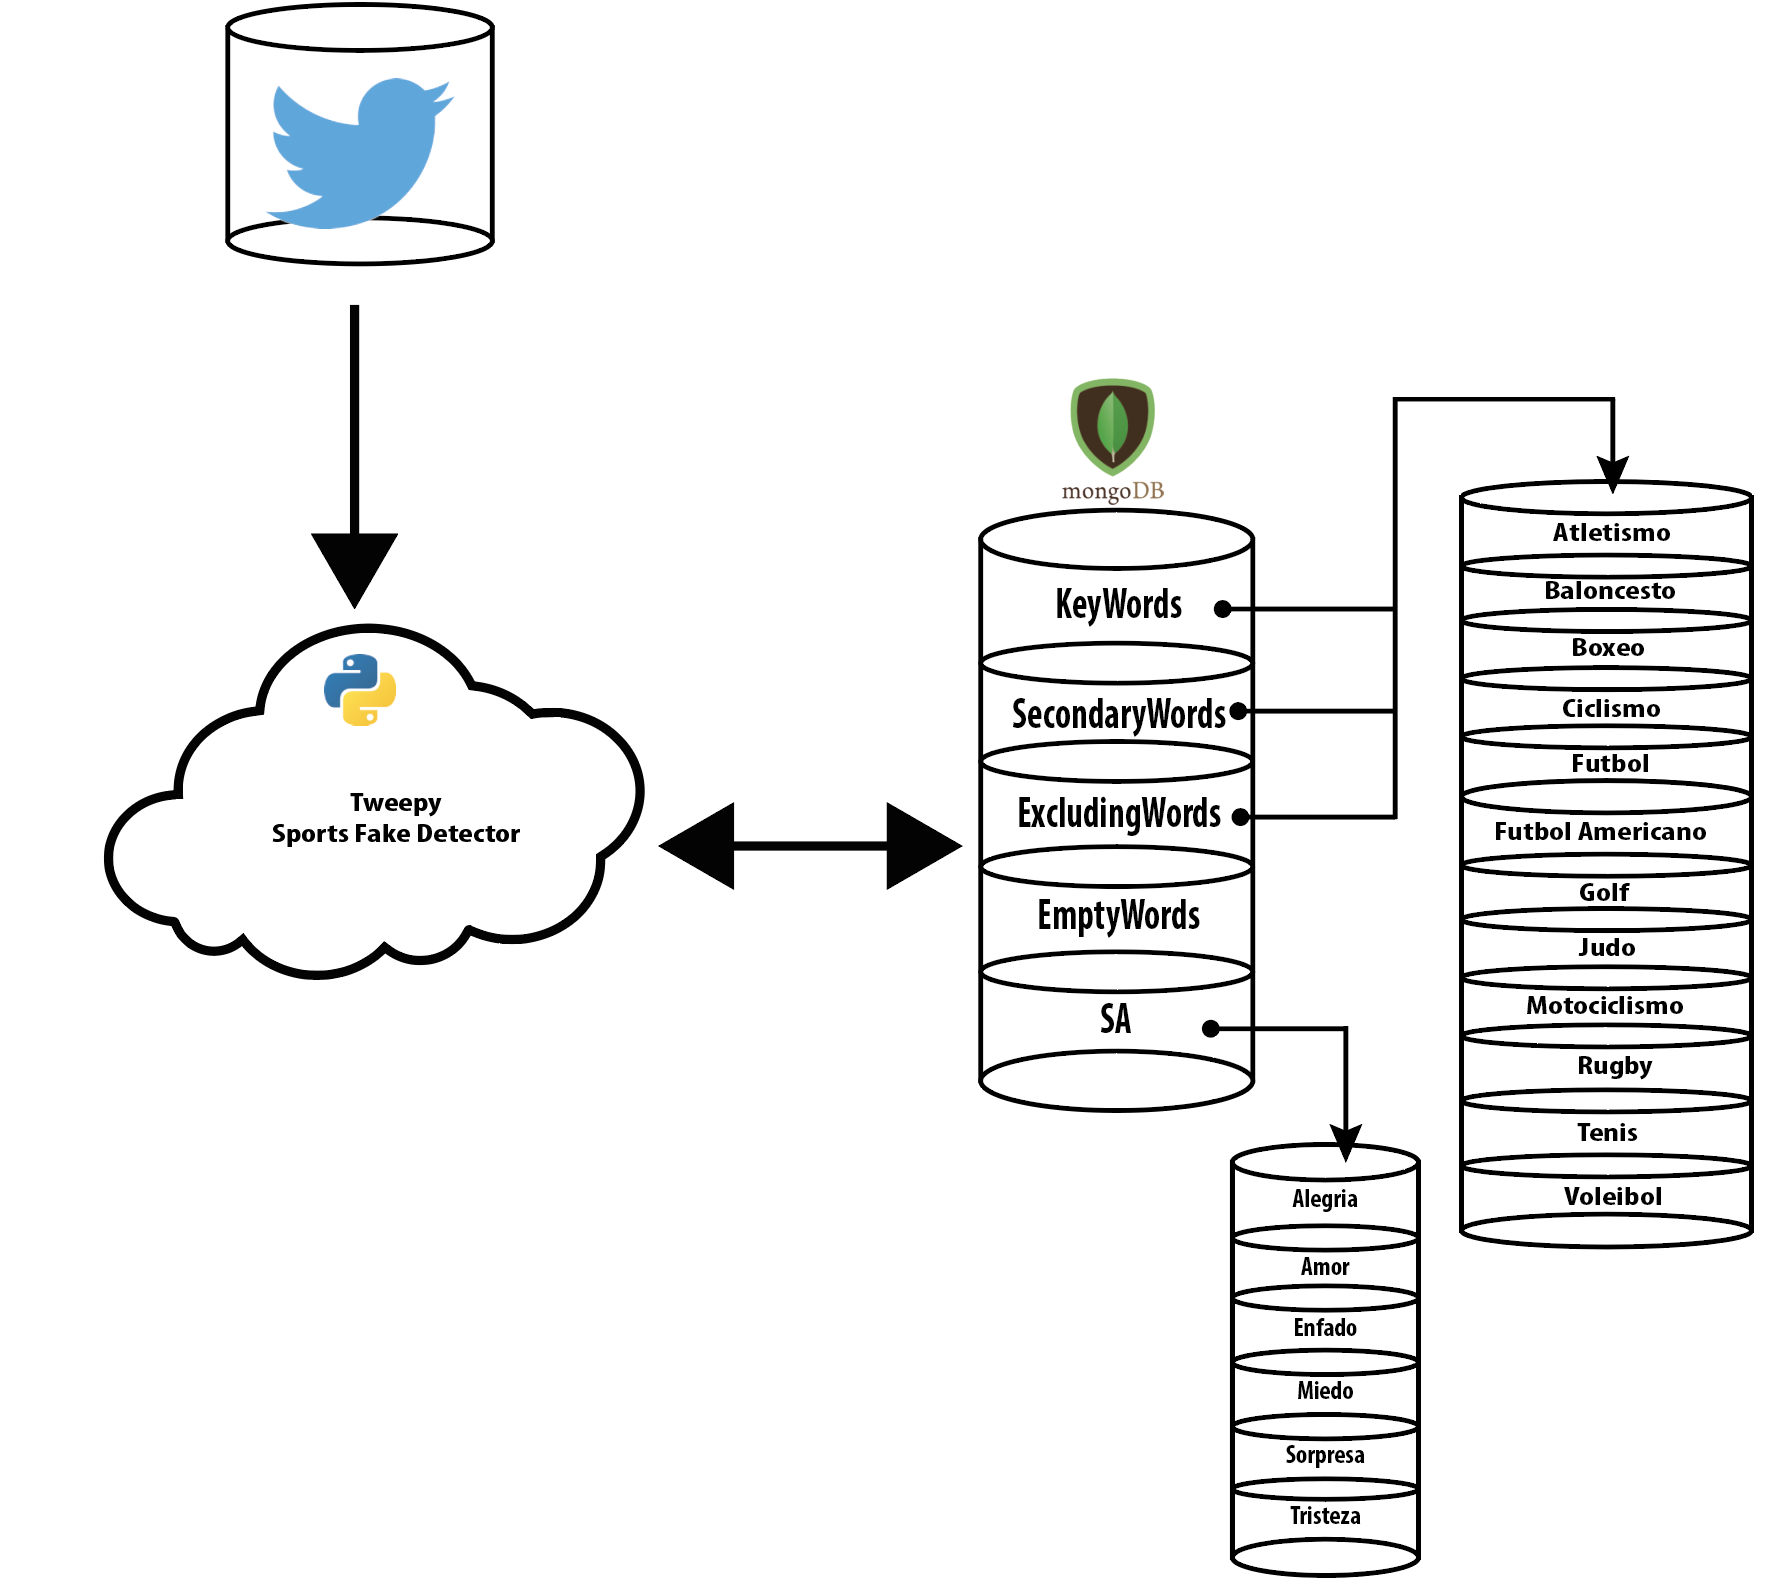
\includegraphics[height=13cm, width=15cm]{imgs/extraccionTwitter.png}
            \caption{Estructura de extracción de tweets y interacción con diccionario}
        \end{figure}
        Donde se puede ver que se extrae la información de twitter a través de la librería tweepy, se proceso con el detector de mentiras y se interacciona con la base de datos donde previamente se habían guardado los diccionarios.\\
        Las tablas de la base de datos son las siguientes:
        \begin{figure}[H]
        \centering
            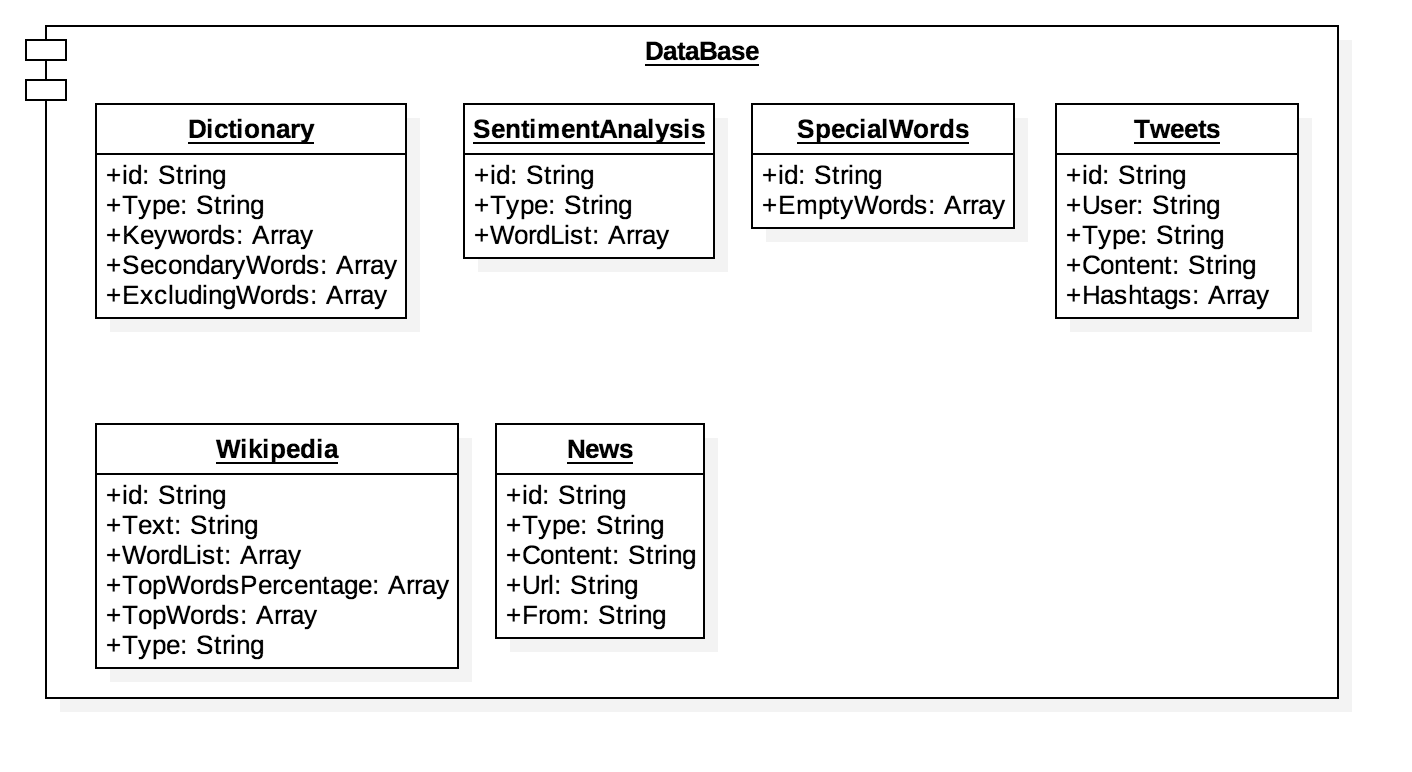
\includegraphics[height=15cm, width=15cm]{imgs/DB.png}
            \caption{Tablas en la base de datos del proyecto}
        \end{figure}
    
        \paragraph{Tweepy 3.5}
            Tweepy es una librería de código abierto para Python que incluye todo el conjunto de funciones necesarias para comunicar con Twitter mediante las API's definidas por este. Las funciones definidas por Tweepy simplifican la conexión y búsquedas con Twitter. Por ejemplo, toda la conexión con Twitter debe estar certificada con un autor y, mientras que por defecto habría que configurar esta conexión mediante otra librería como sería Python-Auth y establecer cada conexión manualmente, Tweepy simplifica esto con unas funciones que simplemente esperan está autenticación como parámetro para poder configurarlo automáticamente. Estos parámetros son 4 tokens necesarios y eb el caso de la búsqueda solo tenemos que indicarle los parámetros que solicita Twitter, toda la complejidad de las conexiones la trata internamente simplificando el trabajo inmensa,ente. Para el proyecto se ha empleado la versión 3.3 de Tweepy.
            \begin{figure}[H]
            	\centering
            	\includegraphics[height=7cm, width=7cm]{imgs/twitter_class.png}
            	\caption{Diagrama de la clase propia Twitter encargada de la comunicación con twitter mediante la librería tweepy}
            \end{figure}
        \paragraph{Wikipedia 1.4.0}
            Está librería se empezó a usar con la finalidad de crear diccionarios automáticamente, simplemente coger todas las palabras que salen de una búsqueda en wikipedia, excluir todos los artículos, proposicionales y palabras que no aportan valor de clasificación.\\
            
            De todas las palabras obtenidas se cogían el 30\% de las palabras más repetidas. Esto permitió empezar a hacer pruebas de los algoritmos pero se descarto por falta de precisión y se empezó a hacer un diccionario propio que ganó riqueza por algunas palabras encontradas gracias a este algoritmo.
            

\newpage    
\subsection{Fase 1 - Clasificación de texto según temática}
    \subsubsection{Concepto}
    	
        {\color{red} 
            TODO
        }
    \subsubsection{Software}
        {\color{red} 
        TODO: Hablar de las librerías python utilizadas, diagrama ...
        }
    
    	\newpage
        \paragraph{Stemmer}
        	Por razones gramaticales, los documentos van a utilizar diferentes formas de una palabra, como jugar, juegan y jugaron o jugador y jugadores. Además, hay familias de palabras derivadas relacionadas con significados similares, como vivir y convivir. En muchas situaciones, parece que sería útil buscar una de estas palabras para devolver documentos que contengan otra palabra en el conjunto.\\
        	
        	El objetivo tanto de la derivación (stemmer) como de la lematización (lemmatization) es reducir las formas flexivas y, a veces, las formas derivadas de una palabra a una forma básica común.\\
        	
        	Sin embargo, las dos palabras difieren en su forma de hacerlo. Stemming usualmente se refiere a un crudo proceso heurístico que elimina los extremos de las palabras con la esperanza de lograr este objetivo correctamente con un alto porcentaje, y a menudo incluye la eliminación de los afijos derivacionales. La lematización generalmente se refiere a hacer las cosas correctamente con el uso de un vocabulario y un análisis morfológico de las palabras, normalmente con el objetivo de eliminar solamente las terminaciones  y devolver la forma base o diccionario de una palabra, lo que se conoce como el lema (lemma).\\
        	
        	Como este trabajo esta en castellano, una lengua muy rica en su vocabulario y derivaciones, se ha optado por usar un Stemmer y no un lematizador dado que se obtienen mejores resultados.\\
        	
        	\begin{figure}[H]
        		\centering
        		\includegraphics[height=13cm, width=15cm]{imgs/stemExampleCode.png}
        		\caption{Código ejemplo utilización VADER}
        	\end{figure}
        	\begin{figure}[H]
        		\centering
        		\includegraphics[height=15cm, width=16cm]{imgs/stemExampleOutput.png}
        		\caption{Output ejemplo utilización VADER}
        	\end{figure}
        	
        	

        \paragraph{Naive Bayes}
        
        	El clasificador Naive Bayes es un clasificador probabilístico que se basa en el teorema de Bayes con suposiciones de independencia. Es una de las técnicas de clasificación de texto más básicas con varias aplicaciones en la detección de spam en el correo electrónico, clasificación de correo electrónico personal, categorización de documentos, detección de lenguaje y detección de sentimiento. \\
        	
        	Como se ha comentado se basa en el teorema de Bayes así que primero lo comentaremos y se usará como ejemplo la clasificación de texto. Se usa para predecir la probabilidad condicional de que un documento pertenezca a una clase P(c{\tiny i}$|$d{\tiny j}) a partir de la probabilidad de los documentos dada la clase P(d{\tiny j} $|$c{\tiny i}) y la probabilidad a priori de la clase en el conjunto de entrenamiento P(c{\tiny i})
        	
        	\begin{figure}[H]
        		\centering
        		\includegraphics[height=5cm, width=5cm]{imgs/naiveBayesEquation.png}
        		\caption{Formula Naive Bayes}
        	\end{figure}
        	
        	Dado que la probabilidad de cada documento P(d{\tiny j}) no aporta información
        	para la clasificación, el término suele omitirse. La probabilidad de un documento
        	dada la clase suele asumirse como la probabilidad conjunta de los términos que
        	aparecen en dichos documentos dada la clase y se calculan como:
        	\begin{figure}[H]
        		\centering
        		\includegraphics[height=5cm, width=5cm]{imgs/multinomialBayesEquation.png}
        		\caption{Formula Multinomial Bayes}
        	\end{figure}
            
        \newpage
        \paragraph{Diccionario}
        	
            {\color{red} 
                TODO
            }

\newpage
\subsection{Fase 2 - Análisis del sentimiento}
    \subsubsection{Concepto}
            {\color{red} 
                TODO
            }
    \subsubsection{Software}
        {\color{red} 
        TODO: Hablar de las librerías python utilizadas, diagrama ...
        }
    
    	\newpage
        \paragraph{Vader Sentiment 3.3}
        
        	VADER (Valence Aware Dictionary and sEntiment Reasoner) es un léxico y una biblioteca de análisis de sentimiento basada en reglas. Sirve como herramienta de análisis de sentimientos basada en reglas que está específicamente adaptada a los sentimientos expresados en las redes sociales.\\
        	
        	 Es completamente de código abierto bajo la [Licencia MIT]. VADER puede incluir el sentimiento de los emoticonos (por ejemplo, :-)), los acrónimos relacionados con el sentimiento (por ejemplo, LOL) y la jerga (por ejemplo, meh).\\
        	 
        	 El método vaderSentiment() devuelve los valores para representar la cantidad de sentimiento negativo, positivo y neutral y también calcula el valor de sentimiento compuesto como un valor con signo para indicar la polaridad del sentimiento general.\\
        	 
        	 A continuación se muestra un ejemplo de utilización de VADER:
        	 \begin{figure}[H]
        	 	\centering
        	 	\includegraphics[height=15cm, width=16cm]{imgs/vaderExampleCode.png}
        	 	\caption{Código ejemplo utilización VADER}
        	 \end{figure}
        	\begin{figure}[H]
        		\centering
        		\includegraphics[height=15cm, width=16cm]{imgs/vaderExampleOutput.png}
        		\caption{Output ejemplo utilización VADER}
        	\end{figure}
        
		\newpage
        \paragraph{TextBlob 0.15.1}
        	TextBlob es una librería de Python (2 y 3) para procesar datos textuales. Proporciona una API simple para adentrarse en tareas comunes de procesamiento del lenguaje natural (NLP), como etiquetado parcial, extracción de frase nominal, análisis de sentimiento, clasificación y traducción.\\
        	
        	En esta fase se ha utilizado esta librería para traducir tweets de otros idiomas y para la clasificación del sentimiento se escogió esta librería porque que ofrece una API simple para acceder a sus métodos y realizar tareas NLP básicas.
        	
        \paragraph{NLTK 3.2.2}
			NLTK (Natural Language Toolkit) es una plataforma líder para construir programas de Python para trabajar con datos de texto natural. Proporciona interfaces fáciles de usar a más de 50 recursos léxicos como WordNet, junto con un conjunto de librerías de procesamiento de texto para clasificación, tokenización, derivación, etiquetado, análisis y razonamiento semántico, envoltorios para bibliotecas de PNL de fuerza industrial, y un foro de discusión activo.\\
			
			Contiene una completa documentación (API). Está disponible para Windows, Mac OS X y Linux. NLTK es un proyecto gratuito y de código abierto que ha sido llamado "una herramienta maravillosa para enseñar y trabajar en lingüística computacional usando Python" y "una biblioteca increíble para jugar con el lenguaje natural".
		\newpage		
        \paragraph{Diccionario}
            {\color{red} 
            TODO: SENTIMENT ANALYSIS WORDS
            }
\newpage
\subsection{Fase 3 - }
    \subsubsection{Concepto}

    \subsubsection{Software}
\end{document}
